\section{Resultados finales y experimentación}

\subsection{Preliminares}

\todo[inline] {Acá explicar que son las diferentes variables que tiene nuestro sistema, alpha, k, K, iters}
\todo[inline] {Explicar medidas que usamos, accuracy, quiza precision/recall}

\subsection{Método de potencia}

Lo primero que nos gustaría ajustar será la cantidad de iteraciones necesarias para el método de la potencia, ya que es algo necesario para todas las mediciones que hagamos. Como adelantamos, para que pasen los tests de la cátedra son necesarias mas de 1000 iteraciones, sin embargo, veremos que con muchas menos iteraciones nuestro accuracy no se modifica. \\

El siguiente experimento fue realizado tomando 10000 muestras de entrenamiento, dejando completamente fijas todas las variables excepto la cantidad de iteraciones. Lo único que intentamos determinar es la cantidad de iteraciones para las cuales la accuracy llega a su máximo. \\

{\centering
    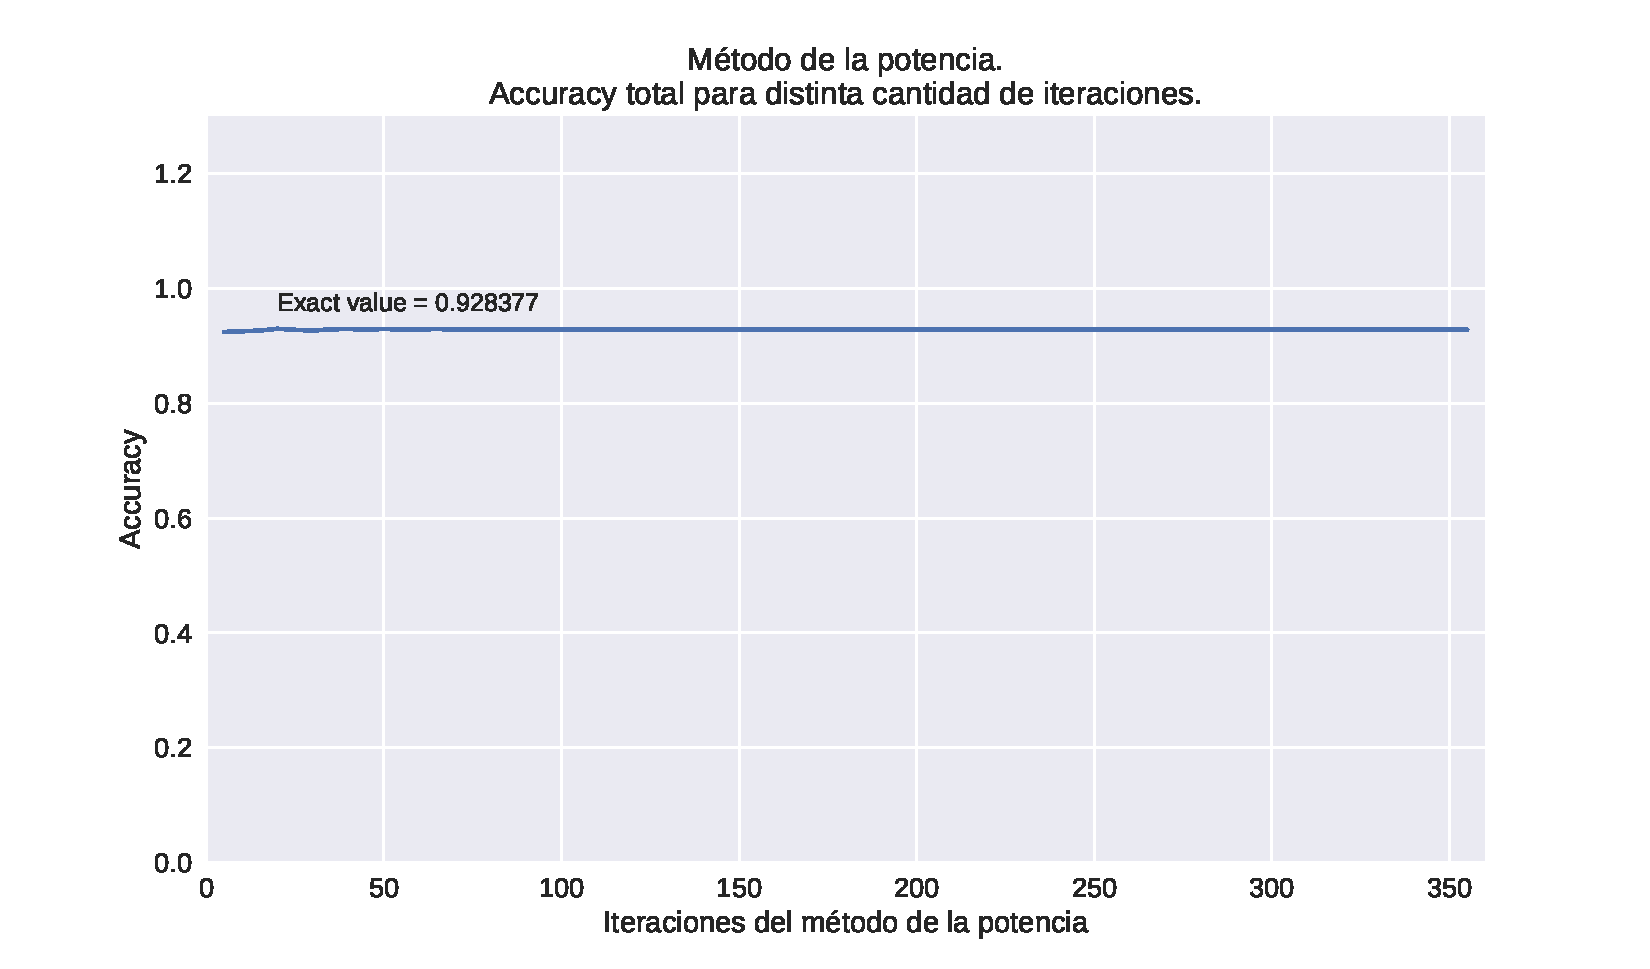
\includegraphics[scale=0.60]{informe/imagenes/potencia/accuracyPorIters.pdf} \\
    \captionof{figure}{Accuracy por cantidad de iteraciones. \\
    Todas las variables fijas \\ }
}
$ $\newline

Como podemos ver, la accuracy se mantiene constante, con la excepción de las cercanías de 10 iteraciones dónde aún son demasiado pocas. Consideramos que no es necesario tomar una cantidad de iteraciones demasiado alta, ya que con aproximadamente 50 parece ser más que suficiente. Es lógico pensar que a mayor cantidad de iteraciones, más tarda nuestro sistema en entrenar. Veamos: \\

\todo[inline]{Gráfico de tiempo con aumento de iteraciones - construccion en proceso - }

$ $ \newline


\subsection{TODO:}

\todo[inline]{Experimentacion con knn variando los k-knn y los K-folds, para encontrar el mejor parametro posible}

\todo[inline]{Experimentacion de tiempo variando la cantidad de imagenes, no hace falta mil experimentos, un par de puntos clave, digamos 100, 1000, 2000, 5000, 10000, 20000, 40000}

\todo[inline]{Comparacion tiempos con, digamos, 10000 training entre knn a secas y con psa.}

\todo[inline]{Comparacion accuaracy y cosas con, digamos, 10000 training entre knn a secas y con psa.}

\todo[inline]{Podemos variar los K-kfolds si la base de entrenamiento es 'chica'}

\todo[inline]{Para entrenamientos con TODAS las imagenes y PSA, QUIZA nos convenga fijar los kfold en, nose, 5, y solo variar los demas parametros. Es RE costoso, (horas) calcular los K folds con un training grande (CON PSA).  Esta piola la idea de agustin de guardarnos en un txt la matriz de covarianza. \\
En limpio, la idea seria: Para 5 folds calcular y guardar las 5 matrices de covarianza, y despues experimentar variando los alphas y los k-knn. Esto seria 'barato' dentro de todo y podrian hacerce un par de graficos. Si hay tiempo variar el k-KFOLD pero lo dejaria para lo ultimo, mejor conseguir resultados concretos antes.}

\todo[inline]{Al final, mostrar resultados de Kaggle con y sin PSA, ir probando con un par de buenos parametros cuando los obtengamos}

\todo[inline]{Me parece muy piola de probar con manuscritos hechos por nosotros. Solo si sobra tiempo!}